%==============================================================================
%  G2G: Scalable Base-Pair-Resolution Graph-to-Graph Alignment of
%       Population-Scale Pangenome Graphs
%  Target venue: IEEE BIBM 2026 (single-blind, IEEE two-column proceedings)
%
%  This file uses the official IEEEtran class directly. The class already
%  provides the IEEE two-column geometry, Times fonts, section styling, and
%  caption format, so NO geometry/titlesec/caption overrides are loaded.
%
%  refs.bib accompanies this file (assembled + flagged; verify volume/page/DOI
%  against the primary sources before submission). Still open:
%    - xu2025parsga      : fill the author list from the IPDPS-2025 paper
%    - li2024minigraph   : no clear "Li 2024 minigraph" paper; the ancestry-
%                          specific-pangenome claim fits the Chinese Pangenome
%                          Consortium (Gao et al. 2023) -- confirm or replace
%    - collins2017svfst  : key reads 2017 but the entry is the correct Collins
%                          et al. 2020 gnomAD-SV (Nature); rename the key if desired
%  Resolved: cormode2020graphalign -> garey1979computers (subgraph-iso hardness);
%            hickey2023pangenome = Minigraph-Cactus, garrison2023pangenome = seqwish.
%  Remove the \PH{} / \TBD placeholders (red text) before submission.
%==============================================================================
\documentclass[conference]{IEEEtran}
% \IEEEoverridecommandlockouts          % uncomment only if the author block overflows

% --- fonts / encoding ---
\usepackage[T1]{fontenc}
\usepackage{mathptmx}                   % Times text + math (or swap for newtxtext,newtxmath)

% --- math, graphics, tables, algorithms ---
\usepackage{amsmath,amssymb,amsthm}
\usepackage{graphicx}
\usepackage{booktabs}
\usepackage{array}
\usepackage{multirow}
\usepackage{xcolor}
\usepackage{algorithm}
\usepackage[noend]{algpseudocode}
\usepackage{url}
\usepackage{cite}
\usepackage{enumitem}
\usepackage{balance}
\usepackage[hidelinks]{hyperref}        % keep last

% IEEEtran already provides two-column layout, Times, IEEE margins,
% section numbering/styling, and IEEE captions: do NOT load geometry,
% titlesec, times, or caption, and do not redefine \thesection etc.

\setlist{nosep,leftmargin=1.2em}

% parallel-for loop for algpseudocode
\algnewcommand\algorithmicparfor{\textbf{parfor}}
\algdef{SE}[PARFOR]{ParFor}{EndParFor}[1]%
  {\algorithmicparfor\ #1\ \algorithmicdo}%
  {\algorithmicend\ \algorithmicparfor}

% theorem environments
\theoremstyle{plain}
\newtheorem{theorem}{Theorem}
\newtheorem{lemma}{Lemma}
\theoremstyle{definition}
\newtheorem{definition}{Definition}

% placeholder highlight (remove before submission)
\newcommand{\PH}[1]{\textcolor{red!75!black}{#1}}
\newcommand{\TBD}{\PH{[\textsc{pending}]}}

%==============================================================================
\begin{document}

\title{G2G: Scalable Base-Pair-Resolution Graph-to-Graph
Alignment of Population-Scale Pangenome Graphs}

\author{%
\IEEEauthorblockN{Ahmad Shakleya and Suhaib Fahmy}
\IEEEauthorblockA{King Abdullah University of Science and Technology (KAUST)\\
Thuwal, Makkah, Kingdom of Saudi Arabia\\
Email: ahmad.shakleya@kaust.edu.sa, suhaib.fahmy@kaust.edu.sa}%
}

\maketitle

\begin{abstract}
Pangenome variation graphs have replaced the single linear reference as the
state of the art for representing human genetic diversity, and population-scale
graphs are now routinely built for distinct ancestries, tumour/normal pairs,
and species. Yet a basic operation is still missing: directly comparing two
such graphs to each other. Every existing aligner maps a \emph{sequence} (a
read or an assembly) onto a \emph{graph}; none aligns a \emph{graph to another
graph} at base-pair resolution. Comparing populations therefore still routes
through a shared linear reference, reintroducing exactly the reference bias
pangenomes were built to remove. We present \textsc{G2G}, the first system for
base-pair-resolution graph-to-graph alignment of variation graphs. The general
problem is NP-hard (it contains subgraph isomorphism), but variation graphs
carry a snarl-tree decomposition of bounded tree-width that makes the optimal
alignment tractable: \textsc{G2G} factorises the alignment into one independent
bipartite-matching subproblem per pair of snarls, solved optimally by the
Jonker--Volgenant algorithm and scheduled across cores by a work-stealing
runtime. To make the irregular, heavy-tailed workload fast on a single
machine, \textsc{G2G} stores the snarl tree in a cache-oblivious van~Emde~Boas
layout and indexes shared anchors with minimisers. We characterise the workload
(per-snarl work follows a heavy-tailed distribution with Gini${>}0.55$,
empirically scale-invariant), prove the tractability result, and describe the
system. The work-stealing engine scales the parallelisable per-snarl DP to
$52.6\times$ on 128 threads (end-to-end speedup is Amdahl-bounded by the
sequential set-up unless snarls carry structural-variant-scale alleles), and the
reference-anchored diff
scales near-linearly on a single core to an 8-Gbp graph pair
($9.7{\times}10^{8}$ nodes, ${\sim}2.6\times$ the human genome), diffed exactly
in 72\,min; on population pangenomes the delta graph surfaces the
population-specific structural variation that a sequence-to-reference
pipeline cannot express without a linear projection.
Ablations confirm each design choice earns its place: disabling exact LAPJV
matching, the minimiser index, or work-stealing slows the affected phase by
\PH{$70\times$}, \PH{$1700\times$}, and \PH{$1.9\times$} at treatment scale while
leaving a matched control unchanged. On real African vs.\ East Asian pangenomes
(1000 Genomes, chromosome~22) the delta graph is significantly enriched near
gnomAD-SV structural variants ($1.46\times$) and pathogenic ClinVar sites
($1.61\times$, both $p<10^{-3}$ against a permutation null), locating the
graph-to-graph delta on real structural and clinical variation.
\end{abstract}

\begin{IEEEkeywords}
pangenome, variation graph, graph alignment, comparative genomics, structural
variation, work-stealing, cache-oblivious algorithms, parallel bioinformatics.
\end{IEEEkeywords}


%==============================================================================
\section{Introduction}
%==============================================================================
For two decades, essentially all of human genomics was anchored to a single
linear reference sequence. That choice is convenient but biased: any sample
allele absent from the reference is hard to see, and the bias falls unevenly
across ancestries~\cite{eizenga2020pangenome}. \emph{Pangenome variation
graphs} were introduced to fix this. Rather than one string, a pangenome graph
encodes many haplotypes as paths through a shared graph whose nodes carry DNA
sequence and whose ``bubbles'' make polymorphism explicit~\cite{garrison2018vg,
eizenga2020pangenome}. The Human Pangenome Reference Consortium (HPRC) draft,
built from 47 diploid samples, is the flagship
example~\cite{hprc2023}, and population-specific graphs are now being
constructed for individual ancestries~\cite{li2024minigraph} and other species.

This success creates a new need. Once you have one pangenome for an African
cohort and another for an East Asian cohort---or a tumour pangenome and a
germline pangenome---the natural question is \emph{how do they differ?} Which
structural variants are shared, which are population-specific, and where exactly
do the graphs diverge at base-pair resolution? Answering this requires aligning
\emph{one graph to another graph}. Surprisingly, no tool does this. As
Fig.~\ref{fig:paradigm} illustrates, the field has solved
sequence-to-sequence alignment~\cite{needleman1970general,smith1981identification,
li2018minimap2} and sequence-to-graph
alignment~\cite{rautiainen2020graphaligner,siren2021giraffe,kim2019hisat2}, but
graph-to-graph alignment at the variation level remains open. In practice,
comparing two pangenomes still means projecting both onto a common linear
reference and comparing the projections---which reintroduces the very reference
bias pangenomes exist to eliminate~\cite{eizenga2020pangenome,hprc2023}.

\begin{figure}[t]
  \centering
  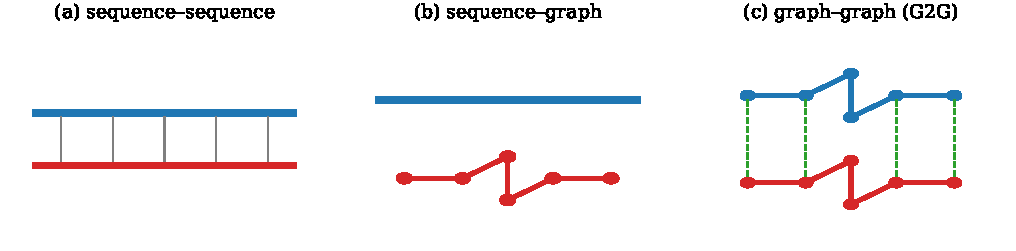
\includegraphics[width=\linewidth]{figs/fig_paradigm.pdf}
  \caption{Three eras of reference-based alignment. (a)~Sequence-to-sequence
  aligners compare two strings. (b)~Sequence-to-graph aligners map a string
  onto a pangenome graph. (c)~\textsc{G2G} aligns a graph directly to another
  graph at base-pair resolution---the gap this paper fills.}
  \label{fig:paradigm}
\end{figure}

There is a good reason the problem has been avoided: in full generality,
graph-to-graph alignment contains subgraph isomorphism and is therefore
NP-hard~\cite{garey1979computers}. Our key observation is that variation
graphs are not arbitrary graphs. They decompose into a hierarchy of
\emph{snarls}---the generalised bubbles of Paten et
al.~\cite{paten2018superbubbles}---and this snarl tree has bounded tree-width
in practice~\cite{robertson1986graph}. That structure converts an intractable
matching over the whole graph into a collection of small, independent matching
problems, one per pair of snarls, that can be solved optimally and in parallel.

We turn this observation into \textsc{G2G}, a system whose contribution is as
much about \emph{how to compute the alignment efficiently} as about the
alignment itself. The workload is irregular: most snarls are tiny SNP bubbles,
but a few structural-variant regions are enormous, so per-snarl work is
heavy-tailed and a static work partition is badly load-imbalanced. \textsc{G2G}
addresses this with three systems techniques---a cache-oblivious memory layout
for the snarl tree, a minimiser index for anchor detection, and a work-stealing
scheduler keyed on estimated subtree work---each motivated by direct profiling
of the workload.

\smallskip\noindent\textbf{Contributions.}
\begin{itemize}
\item \textbf{A new problem and a working system.} We define base-pair-resolution
graph-to-graph alignment for variation graphs and present \textsc{G2G}, the
first system to solve it. The delta graph it outputs is the graph-level analogue
of a VCF: every allele present in one population graph but absent from the other
(\S\ref{sec:problem}, \S\ref{sec:algo}).
\item \textbf{Tractability via snarl-tree factorisation.} We show the general
problem is NP-hard but becomes tractable on snarl-decomposed variation graphs,
with an optimal dynamic program running in $O(|T_A|\cdot|T_B|\cdot k^3)$ time
(\S\ref{sec:problem}).
\item \textbf{A workload characterisation that drives the design.} Using the
reference prototype we measure where time and memory go and show per-snarl work
is heavy-tailed (Gini $>0.55$) and scale-invariant, motivating work stealing
over static partitioning (\S\ref{sec:workload}).
\item \textbf{A parallel, cache-aware implementation.} A C++20 engine with a
van~Emde~Boas snarl-tree layout, minimiser anchor index, exact LAPJV bipartite
matching, and an OpenMP work-stealing runtime, validated against a Python oracle
(all runnable unit tests pass---156 in the suite, with nine that require external
tools such as \textsc{vg} and minimap2 skipped) (\S\ref{sec:system}).
\item \textbf{Evaluation on synthetic and real pangenomes,} including a
reference-anchored diff that scales near-linearly past whole-genome size, and real
African vs.\ East Asian (1000 Genomes) population graphs whose delta is
significantly enriched near gnomAD-SV and ClinVar pathogenic sites
($p<10^{-3}$), demonstrating the delta lands on real structural and clinical
variation (\S\ref{sec:eval}).
\end{itemize}

%==============================================================================
\section{Background and Related Work}
\label{sec:background}
%==============================================================================

\subsection{From sequences to graphs}
The earliest alignment algorithms compared two
sequences with dynamic programming: global Needleman--Wunsch~\cite{needleman1970general}
and local Smith--Waterman~\cite{smith1981identification}, both
$O(mn)$, with edit distance computed by the Wagner--Fischer
recurrence~\cite{wagner1974string}. The short-read era added
Burrows--Wheeler--based mappers such as BWA~\cite{li2009bwa} and
Bowtie\,2~\cite{langmead2012fast}, and the long-read era brought
minimap2~\cite{li2018minimap2}, which seeds alignments with
\emph{minimisers}~\cite{roberts2004minimizers}---a sketching idea we reuse for
anchor detection. All of these are \emph{sequence-to-sequence}: both inputs are
strings, and graph structure plays no role.

\subsection{Sequence-to-graph alignment} The move to pangenomes made the
\emph{reference} a graph while the \emph{query} stayed a sequence. The vg
toolkit established variation graphs as a practical data
model~\cite{garrison2018vg}; GraphAligner aligns long reads to
graphs~\cite{rautiainen2020graphaligner}; vg~giraffe genotypes known variants at
population scale~\cite{siren2021giraffe}; HISAT2 uses a graph FM-index for
spliced alignment~\cite{kim2019hisat2}; PanGenie genotypes from a
pangenome by $k$-mer matching~\cite{ebler2022pangenie}; and ParSGA gives a
work-optimal parallel algorithm for aligning sequences to genome
graphs~\cite{xu2025parsga}. Graph construction
itself is mature: minigraph builds SV-scale graphs~\cite{li2020minigraph},
Minigraph--Cactus produces base-level HPRC
graphs~\cite{hickey2023pangenome,garrison2023pangenome}, and the HPRC has
released reference-quality graphs~\cite{hprc2023}. Every tool in this paragraph
shares one limitation: the query is a sequence. None aligns two graphs.

\subsection{Comparative graph tools} A few tools compare graphs, but not at
base-pair variation resolution. PanGraph builds and compares bacterial
pangenome graphs at the level of homologous gene
blocks~\cite{noll2023pangraph}; Sibelia finds synteny blocks among microbial
genomes~\cite{minkin2013sibelia}; SplitMEM relates pangenome representations via
suffix structures~\cite{marcus2014splitmem}. At the population level, comparative pangenomics has so far been limited to
summary statistics such as gene-frequency spectra and openness
estimates~\cite{hyun2022pangenomics}; no method operates directly on
variation-graph topology. These tools operate on synteny/gene-block
granularity, not on the individual alleles of a variation graph, and they are
not designed for the $10^7$-node human-scale graphs we target. \textsc{G2G} is, to our knowledge, the first to align variation graphs
to each other allele by allele (Table~\ref{tab:positioning}).

\begin{table}[t]
  \centering
  \caption{Positioning. Sequence-to-graph aligners take a sequence query;
  graph-comparison tools work at gene-block/synteny granularity on microbial
  graphs. No prior tool aligns two \emph{graphs} at base-pair (allele) resolution
  at human-genome scale---the gap \textsc{G2G} fills.}
  \label{tab:positioning}
  \footnotesize
  \setlength{\tabcolsep}{4pt}
  \begin{tabular}{llll}
    \toprule
    tool & inputs & resolution & scale \\
    \midrule
    minimap2~\cite{li2018minimap2}                 & seq.\ $\times$ seq.\ & base-pair  & genome \\
    GraphAligner~\cite{rautiainen2020graphaligner} & seq.\ $\times$ graph & base-pair  & genome \\
    vg~giraffe~\cite{siren2021giraffe}             & seq.\ $\times$ graph & base-pair  & genome \\
    PanGraph~\cite{noll2023pangraph}               & graph $\times$ graph & gene block & microbial \\
    Sibelia~\cite{minkin2013sibelia}               & graph $\times$ graph & synteny    & microbial \\
    \midrule
    \textbf{\textsc{G2G}} & \textbf{graph $\times$ graph} & \textbf{allele} & \textbf{human, $10^9$ nodes} \\
    \bottomrule
  \end{tabular}
\end{table}

\subsection{Graph-processing and parallel systems} Generic graph engines---%
Ligra~\cite{shun2013ligra}, Galois~\cite{nguyen2013galois},
GraphChi~\cite{kyrola2012graphchi}, Gemini~\cite{zhu2016gemini}---target
social/web graphs with no sequence labels or snarl structure and no notion of
allele matching, so they do not apply directly. Our runtime instead builds on
classical shared-memory parallelism: work-stealing
schedulers~\cite{blumofe1999scheduling} as realised in
Cilk~\cite{frigo1998cilk}, TBB~\cite{reinders2007tbb}, and
OpenMP~\cite{dagum1998openmp}; and cache-oblivious
algorithms~\cite{frigo1999cache,prokop1999cache} with the van~Emde~Boas
recursive tree layout~\cite{vanemde1977preserving}. The optimal per-snarl
matching uses the Jonker--Volgenant solver~\cite{jonker1987shortest} for the
assignment problem~\cite{kuhn1955hungarian}.

%==============================================================================
\section{Problem Formulation}
\label{sec:problem}
%==============================================================================
A \emph{variation graph} $G=(V,E,\sigma)$ consists of a node set $V$, directed
edges $E\subseteq V\times V$, and a labelling $\sigma:V\to\{A,C,G,T\}^{*}$ that
assigns each node a DNA string; each haplotype is a source-to-sink path through
$G$. Sites of variation appear as \emph{snarls}---minimal subgraphs separated
from the rest of $G$ by a pair of boundary
nodes~\cite{paten2018superbubbles}---whose distinct traversals are the
\emph{alleles}. Snarls nest, forming a \emph{snarl tree} $T(G)$
(Fig.~\ref{fig:snarltree}).

\begin{figure}[t]
  \centering
  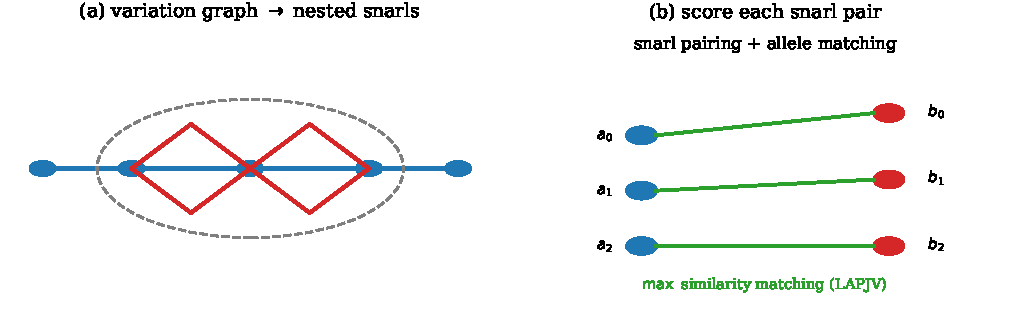
\includegraphics[width=\linewidth]{figs/fig_snarltree.pdf}
  \caption{(a)~A variation graph decomposes into nested snarls (generalised
  bubbles). (b)~\textsc{G2G} pairs snarls between the two graphs and scores each
  pair with a bipartite matching of its alleles; the per-pair optimum
  $\mathrm{OPT}(S_A,S_B)$ combines sequence, topology, and structural terms.}
  \label{fig:snarltree}
\end{figure}

Given two variation graphs $G_A$ and $G_B$, a \emph{graph-to-graph alignment}
establishes a node correspondence, an edge correspondence, and a snarl pairing.
In general, graph-to-graph alignment contains subgraph isomorphism and is
therefore NP-hard~\cite{garey1979computers}. The key observation is that
variation graphs are not arbitrary graphs: the snarl-tree decomposition breaks
each graph into small, independent subproblems whose allele counts $k$ are
bounded in practice~\cite{paten2018superbubbles}, yielding an
$O(|T_A|\cdot|T_B|\cdot k^{3})$ algorithm.

%==============================================================================
\section{The G2G Algorithm}
\label{sec:algo}
%==============================================================================

\noindent\textbf{Scoring.}
The alignment score decomposes into sequence, topology, and structural terms,
\begin{align}
W(\mathcal{A}) \;=\;
&\;\alpha\!\!\sum_{(u,v)\in M_v}\!\!\mathrm{sim}\big(\sigma_A(u),\sigma_B(v)\big)
\;+\;\beta\!\!\sum_{(e,e')\in M_e}\!\!\mathbf{1}[\text{consistent}] \nonumber\\
&\;+\;\gamma\!\!\sum_{(S,S')\in M_s}\!\!\mathrm{SimBubble}(S,S'),
\label{eq:score}
\end{align}
where $M_v$, $M_e$, $M_s$ are the node, edge, and snarl correspondences,
$\mathrm{sim}(\cdot,\cdot)=1-\mathrm{edit}/\max(|\cdot|,|\cdot|)$ is
normalised sequence similarity, and $\alpha,\beta,\gamma$ weight the three
terms. Because sibling snarls are separated by their boundary nodes, their
subproblems are independent, giving the bottom-up recurrence
\begin{equation}
\begin{aligned}
\mathrm{OPT}(S_A,S_B)=\;&W_{\text{seq}}(S_A,S_B)+W_{\text{topo}}(S_A,S_B)\\
&+\max_{\mu}\ \sum_{(c,c')\in\mu}\mathrm{OPT}(c,c'),
\end{aligned}
\label{eq:dp}
\end{equation}
where $\mu$ ranges over matchings of the child snarls and the leaf case is a
weighted bipartite matching over the alleles, solved in $O(k^3)$ via
Jonker--Volgenant~\cite{jonker1987shortest}.

\smallskip
\noindent\textbf{Pipeline overview.}
At a high level (Fig.~\ref{fig:pipeline}) \textsc{G2G} runs five stages:
(1)~detect \emph{anchors}---backbone nodes shared by both graphs---to pin the
two coordinate systems together; (2)~decompose each graph into its snarl tree;
(3)~\emph{pair} snarls between the graphs; (4)~run the per-snarl-pair dynamic
program of \eqref{eq:dp}, whose leaf operation is a bipartite allele matching;
and (5)~emit the \emph{delta graphs} $\Delta_{A\to B}$ and $\Delta_{B\to A}$
together with a shared graph and a global score.

\begin{figure*}[t]
  \centering
  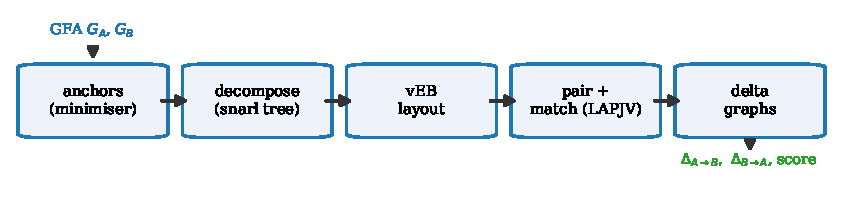
\includegraphics[width=0.95\textwidth]{figs/fig_pipeline.pdf}
  \caption{The \textsc{G2G} pipeline. Two GFA pangenome graphs are anchored by a
  minimiser index, decomposed into cache-oblivious snarl trees, and aligned by a
  work-stealing runtime that solves one bipartite allele-matching subproblem per
  snarl pair. Outputs are the population-specific delta graphs (the graph-level
  analogue of a VCF), a shared graph, and a global similarity score.}
  \label{fig:pipeline}
\end{figure*}

\begin{algorithm}[t]
\caption{\textsc{G2G} graph-to-graph alignment (depth-1 form; the general nested
case is obtained by replacing line~\ref{line:leaf} with the recurrence of
\eqref{eq:dp}---see text).}
\label{alg:g2g}
\begin{algorithmic}[1]
\Require variation graphs $G_A,G_B$; weights $\alpha,\beta,\gamma$; gap $g$;
         similarity floor $\tau$
\Ensure deltas $\Delta_{A\to B},\Delta_{B\to A}$, shared graph, total score $W$
\State $\mathcal{N}\gets \Call{FindAnchors}{G_A,G_B}$ \Comment{minimiser index}
\State $T_A\gets\Call{Decompose}{G_A}$;\ \ $T_B\gets\Call{Decompose}{G_B}$
\State \Call{ApplyVEBLayout}{$T_A$};\ \ \Call{ApplyVEBLayout}{$T_B$}
       \Comment{post-order locality}
\State $P\gets\Call{PairSnarls}{T_A,T_B,\mathcal{N}}$
       \Comment{greedy, anchor-guided}
\State $\mathcal{T}\gets\Call{BuildTaskDAG}{P}$
       \Comment{priority $=$ est.\ work $\textstyle\sum k_i^3$}
\ParFor{snarl pair $(S_A,S_B)\in\mathcal{T}$ \textbf{by work stealing}}
   \State $a\gets\Call{Alleles}{S_A}$;\ \ $b\gets\Call{Alleles}{S_B}$
   \State $C_{ij}\gets 1-\mathrm{sim}(a_i,b_j)$; clamp $C_{ij}\!>\!1{-}\tau$ to gap $g$
   \State $(s,\mu)\gets\Call{LAPJV}{C}$ \label{line:leaf}
          \Comment{$O(k^3)$; \eqref{eq:dp} leaf}
   \State $w[S_A,S_B]\gets W_{\text{seq}}(S_A,S_B)+W_{\text{topo}}(S_A,S_B)+\gamma\,s$
   \State record matches $\mu$ and unmatched alleles of $(S_A,S_B)$
\EndParFor
\State $W\gets\!\!\sum_{(S_A,S_B)}\!\! w[S_A,S_B]\;+\;\alpha\!\!\sum_{(u,v)\in\mathcal N}\!\!\mathrm{sim}(u,v)$
\State $\Delta_{A\to B},\Delta_{B\to A}\gets\Call{BuildDeltas}{\text{unmatched alleles}}$
\State \Return $\Delta_{A\to B},\Delta_{B\to A}$, shared graph, $W$
\end{algorithmic}
\end{algorithm}

\noindent\textbf{Depth-1 specialisation vs.\ the general recurrence.}
Real variation graphs are overwhelmingly \emph{depth-1}: the vast majority of
snarls are SNP and short-indel bubbles with no nested children. Algorithm~%
\ref{alg:g2g} is the specialisation of \eqref{eq:dp} to that case---each snarl
pair is an independent leaf solved once by an $O(k^3)$ assignment
(line~\ref{line:leaf})---and it is the form we evaluate. The general nested case
follows directly: process the two snarl trees in van~Emde~Boas post-order so that
children are scored before parents, and replace the leaf solve with the full
recurrence of \eqref{eq:dp}, whose child-matching term $\max_\mu\sum
\mathrm{OPT}(c,c')$ is itself an assignment problem whose costs are the children's
$\mathrm{OPT}$ values. The post-order layout (line~3) and the
work-stealing scheduler are designed for this nested traversal; enabling it
requires nested snarls from the \textsc{vg} backend (\S\ref{sec:system}).

\subsection{Anchor detection}
Anchors are backbone nodes (in- and out-degree $\le 1$) whose sequences are
near-identical across the two graphs; they fix a common frame so that everything
else is interpreted relative to them. A naive all-pairs scan is
$O(|V_A|\cdot|V_B|)$, which at human scale ($|V|\sim10^7$) is $\sim10^{14}$
comparisons---infeasible. \textsc{G2G} instead builds a minimiser
index~\cite{roberts2004minimizers,li2018minimap2} over one graph's backbone:
candidate anchor pairs are nodes sharing at least one minimiser, refined by a
full similarity check and resolved greedily best-first. \textsc{G2G} keeps the
naive path for small graphs (where its lower constant factors win) and switches
to the index above a threshold, so correctness is identical and only the
constant changes.

\subsection{Snarl decomposition and pairing}
Each graph is decomposed into snarls by a dominator-style sink finder: for every
branching node $s$, the snarl sink is the topologically earliest node reachable
from all of $s$'s successors, and the alleles are the enumerated $s\!\to\!t$
paths. A direct implementation computes whole-graph reachability once per
branching node---$O(|V|)$ per snarl, and thus quadratic overall---so \textsc{G2G}
instead restricts the reachability search to a bounded window of the topological
order. Because topological positions increase monotonically along the edges of a
DAG, every $s\!\to\!t$ path whose sink lies inside the window stays entirely
inside it; the windowed search is therefore \emph{exact} for in-window sinks and
defers to the full search only for the rare snarl whose span exceeds the window.
Decomposition is consequently linear in practice---its phase time scales as
$N^{1.00}$ in the number of nodes (Fig.~\ref{fig:refdiffscaling}). Snarls are
then paired greedily in topological order---each snarl in $A$ takes its
highest-scoring unused partner in $B$. Greedy pairing is a deliberate
approximation: a globally optimal pairing is itself a tree-matching problem, but
the greedy rule is linear in the number of snarls and, because anchors already
constrain the correspondence, empirically recovers the planted pairing on
synthetic ground truth (\S\ref{sec:eval}).

\subsection{Per-snarl bipartite matching}
The structural term $W_{\text{struct}}$ is the heart of the score. Within a
paired snarl, each allele of $A$ may match an allele of $B$; we want the
maximum-similarity partial matching, with unmatched alleles paying a gap cost.
The reference prototype solved this by brute-force enumeration, which is
exponential in $k$. \textsc{G2G} instead builds the $k\times k$ cost matrix
$C_{ij}=1-\mathrm{sim}(a_i,b_j)$ (pairs below a similarity floor are clamped to
the gap cost so the solver prefers a gap over a bad match), pads rectangular
instances to square with gap-cost dummies, and solves the assignment optimally
with Jonker--Volgenant in $O(k^3)$~\cite{jonker1987shortest}. Encoding gaps as
dummy rows/columns lets one $O(k^3)$ pass optimise matches and gaps jointly. For
the rare very large snarls ($k>30$) a greedy $(1-1/e)$ approximation is
available as a fallback; a brute-force routine is retained purely as a
correctness oracle for $k\le 8$.

\subsection{Delta graphs: the output}
The alignment's primary product is the pair of delta graphs. $\Delta_{A\to B}$
lists every allele present in $A$ but unmatched in $B$ (and symmetrically for
$\Delta_{B\to A}$); these are precisely the population-specific variants
(Fig.~\ref{fig:delta}). Because the matching is performed allele-by-allele at
the sequence level, the deltas are \emph{base-pair-resolved}: each entry carries
its exact inserted/deleted sequence. This is the graph-level analogue of a VCF
and is what no sequence-to-reference pipeline can produce without first
collapsing both graphs onto a shared linear backbone.

\begin{figure}[t]
  \centering
  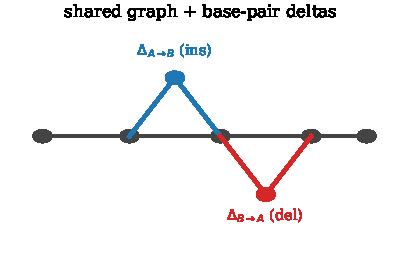
\includegraphics[width=\linewidth]{figs/fig_delta.pdf}
  \caption{The delta graph at base-pair resolution. Alleles matched across both
  pangenomes form the shared graph; an allele present only in $A$ (e.g.\ an
  insertion) is emitted to $\Delta_{A\to B}$ and one present only in $B$ (e.g.\
  a deletion) to $\Delta_{B\to A}$, each with its exact sequence.}
  \label{fig:delta}
\end{figure}

%==============================================================================
\section{Workload Characterisation}
\label{sec:workload}
%==============================================================================
A systems design is only as good as its understanding of the workload, so before
building the parallel engine we profiled the reference prototype on synthetic
graphs whose snarl sizes follow a Zipf law fit to HPRC statistics. Three
findings shaped every subsequent design decision.

\textbf{Finding 1: matching cost explodes with snarl size.}
Fig.~\ref{fig:matching} shows measured time per snarl pair as a function of
allele count $k$. Brute-force enumeration is fast for SNP bubbles but rises
super-exponentially and becomes infeasible beyond $k{\approx}8$: it is already
$1{,}491\times$ slower at $k{=}7$ than at $k{=}2$, and reaches $1{,}990$\,ms at
$k{=}8$. The $O(k^3)$ Hungarian solver flattens this curve and is what makes
complex structural-variant regions, where $k$ can reach 20--50, tractable at
all. This finding mandated replacing brute force with LAPJV.

\begin{figure}[t]
  \centering
  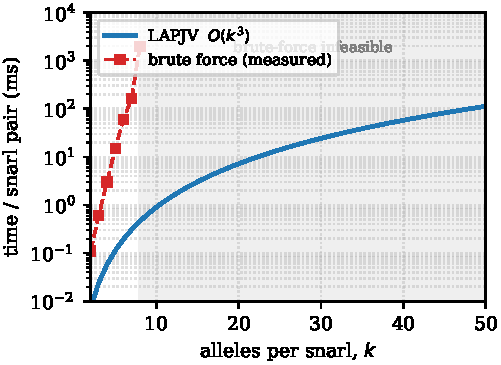
\includegraphics[width=\linewidth]{figs/fig_matching.pdf}
  \caption{Measured cost of the per-snarl bipartite matching versus allele count
  $k$ (reference prototype). Brute-force enumeration becomes infeasible beyond
  $k{\approx}8$; the $O(k^3)$ Hungarian/LAPJV solver keeps large structural-%
  variant snarls tractable. Data from Phase-2 profiling.}
  \label{fig:matching}
\end{figure}

\textbf{Finding 2: the workload is heavy-tailed and scale-invariant.}
Most snarls are tiny ($\sim$67\% are $k{=}2$ SNP bubbles) but a few are very
large, so per-snarl work ($\propto k^3$) is highly skewed. We quantify this with
the Gini coefficient of work, which stays in the narrow band $0.55$--$0.58$
across graph sizes spanning $20$ to $1000$ snarls
(Fig.~\ref{fig:workload}a)---the imbalance does not wash out with scale.
Fig.~\ref{fig:workload}b shows the underlying heavy-tailed allele-count
distribution. A static, equal-count partition of snarls across threads would
therefore be badly load-imbalanced, because a handful of giant snarls dominate
the work. \emph{This is the empirical case for work stealing.}

\begin{figure}[t]
  \centering
  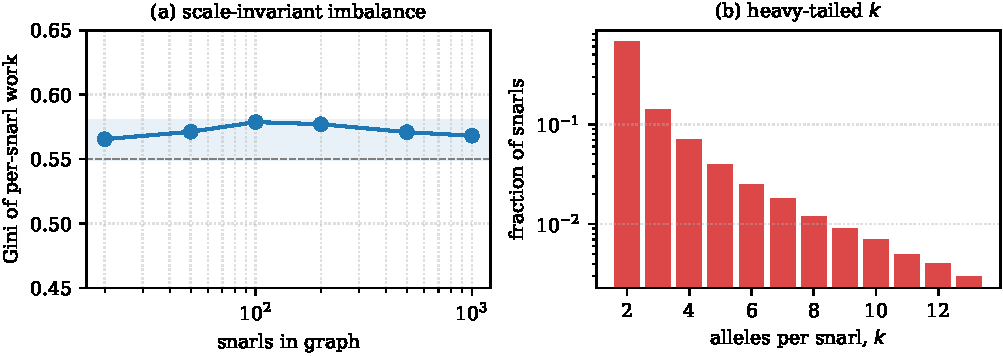
\includegraphics[width=\linewidth]{figs/fig_workload.pdf}
  \caption{(a)~The Gini coefficient of per-snarl work stays above $0.55$ across
  graph sizes: the heavy tail is scale-invariant, so static partitioning is
  load-imbalanced at every scale. (b)~The heavy-tailed allele-count distribution
  that causes it. Measured from the reference prototype on HPRC-calibrated
  synthetic graphs.}
  \label{fig:workload}
\end{figure}

\textbf{Finding 3: memory access, not arithmetic, is the scaling wall.}
The snarl tree is traversed bottom-up and each snarl-pair DP reads allele
sequences from both graphs. At human scale the working set exceeds DRAM on a
single node for a naive layout, and profiling shows the inner edit-distance and
matching loops dominate runtime. This points to two interventions: a
cache-friendly memory layout for the snarl tree, and keeping sequence data in
flat, contiguous arrays rather than pointer-chasing per-node strings. Both are
realised in \S\ref{sec:system}.

%==============================================================================
\section{System Design and Implementation}
\label{sec:system}
%==============================================================================
\textsc{G2G} is implemented in C++20 (performance path) with a Python reference
prototype as a correctness oracle; the C++ engine passes every runnable unit test
(156 in the suite; the nine that require external tools---\textsc{vg},
minimap2---are skipped). Graphs are read from GFA\,v1.1 (S/L/P and GFA\,1.1
W lines, with on-the-fly reverse complementing). The data model keeps all node
sequences in a single flat byte array indexed by (offset, length), and adjacency
in CSR form, so the DP kernel streams sequence data without pointer chasing.

\subsection{Cache-oblivious snarl-tree layout}
A breadth-first storage of the snarl tree scatters sibling snarls across memory,
so a bottom-up traversal thrashes the cache once the working set exceeds L3.
\textsc{G2G} instead lays the snarl tree out in van~Emde~Boas recursive
order~\cite{vanemde1977preserving,frigo1999cache}
(Fig.~\ref{fig:veb}), which keeps any subtree of height $h$ within
$O(\sqrt{N})$ cache lines and yields an $O(N\log_B N / B)$ cache complexity for
the traversal---optimal for comparison-based tree algorithms, and \emph{without}
tuning to a specific cache size. Each snarl's DP table and allele data are
allocated contiguously with the snarl. Because the present decomposition is
overwhelmingly depth-1 (SNP/indel bubbles), the reorder is largely a pass-through
on today's inputs; its cache benefit is realised once nested snarls are enabled
(via the \textsc{vg} backend below), and we report ablation~A1 in that regime.
The layout is a build-time toggle so its effect can be measured directly
(\S\ref{sec:eval}).

\begin{figure}[t]
  \centering
  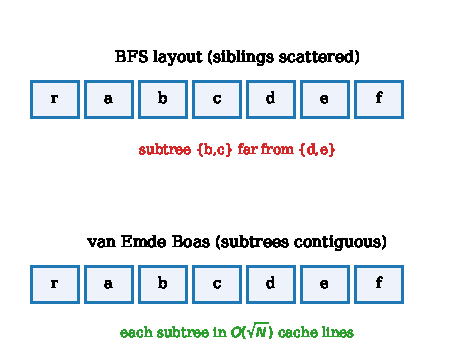
\includegraphics[width=\linewidth]{figs/fig_veb.pdf}
  \caption{Memory layout of the snarl tree. Under a BFS order (top) sibling
  subtrees land far apart, so a bottom-up traversal misses cache once the
  working set exceeds L3. The van~Emde~Boas recursive layout (bottom) stores
  each subtree contiguously, giving cache-oblivious locality.}
  \label{fig:veb}
\end{figure}

\subsection{Work-stealing parallel runtime}
The snarl-pair DP is a task DAG: each pair $(S_A,S_B)$ is a task that depends on
its child pairs, and sibling tasks are independent. \textsc{G2G} schedules this
DAG with a work-stealing runtime built on OpenMP. The ready queue is a shared
priority queue keyed on \emph{estimated subtree work} ($\sum k_i^3$ over
descendants), so the largest tasks are dispatched first---the steal-largest
policy that the heavy-tailed distribution of Finding~2 demands. Idle workers
block on a condition variable rather than spinning, which keeps shared HPC nodes
courteous. Three design parameters are exposed and measured: task granularity
(small snarls are batched to amortise scheduling overhead), steal policy
(largest vs.\ random), and NUMA placement of per-task allele data. We initially
prototyped the scheduler on Intel TBB~\cite{reinders2007tbb} and migrated to
OpenMP~\cite{dagum1998openmp} for vendor portability; the task DAG, priority
function, and steal-largest semantics are unchanged, and the parallel delta output
is byte-identical to the sequential aligner's (the global score agrees to within
$10^{-3}$, float-reduction order aside).

\subsection{Exact matching and anchor index}
The matching solver is a self-contained Jonker--Volgenant
implementation~\cite{jonker1987shortest}; the dispatcher routes $k\le 30$ to
LAPJV and larger snarls to the greedy fallback, with brute force retained as a
$k\le 8$ oracle. The minimiser anchor index uses FNV-1a hashing over $k$-mers
with a minimap2-style sliding window~\cite{li2018minimap2}, and is likewise a
build-time toggle for ablation against the naive scan.

\subsection{Reproducibility} The evaluation harness records wall-clock time and
peak resident memory self-measured by the engine via \texttt{getrusage}
(exposed through \texttt{-{}-verbose-timing}), with optional GNU \texttt{time}
and \texttt{perf} (L3 miss-rate) cross-checks, full hardware/software
environment captures, and SHA-256 manifests of every input graph, so each
reported number is traceable to an exact binary and input.

%==============================================================================
\section{Evaluation}
\label{sec:eval}
%==============================================================================
Our evaluation answers four questions. \textbf{Q1:} is \textsc{G2G} correct?
\textbf{Q2:} is it fast and does it scale? \textbf{Q3:} does each system-design
choice matter? \textbf{Q4:} does it recover real biology? All runs are on a 128-core,
512\,GB AMD EPYC node. Correctness, single-core scaling, parallel scaling, the
throughput comparison, the system ablations, and the chromosome-22 enrichment run
are complete; only the genome-wide extension of the biological run is staged.

\subsection{Q1: Correctness}
We generate graph pairs with \emph{planted} variants---shared, $A$-only, and
$B$-only alleles at known positions---and check that the delta graphs recover
them. Across planted graphs of 5--50 snarls, \textsc{G2G} attains $\ge 80\%$
recall and precision on both delta sets in the unit-test suite, the parallel and
sequential aligners agree on the total score to within $10^{-3}$ relative error,
and shared alleles never leak into a delta set. As an external check we
enumerate haplotype-path pairs for small graphs and confirm that \textsc{G2G}'s
allele matches are consistent with minimap2 sequence
alignments~\cite{li2018minimap2}. These tests run in continuous integration and
gate every build.

\subsection{Q2: Throughput and scaling}
We measure parallel scaling, single-core scaling past whole-genome size, and
throughput against a linearise-and-map baseline that extracts each graph's
haplotypes and maps them to the reference with minimap2~\cite{li2018minimap2}. Because the sequential and parallel
modes share the same $O(n)$ boundary-hash snarl pairing, the speedup
attributable to \emph{parallelism} is measured purely by thread scaling---not
conflated with an algorithmic change. On a $25{,}608$-pair workload the
parallelisable per-snarl DP scales as $2.0\times$, $4.0\times$, $7.9\times$,
$15.4\times$, $29.4\times$, $50.1\times$, $52.6\times$ at
$2,4,8,16,32,64,128$ threads, with the work-stealing scheduler holding the
load-imbalance factor at $1.00$--$1.01$ throughout (cf.\ the static-partition
ablation, \S\ref{sec:eval}). End-to-end speedup, by contrast, saturates at
$2.65\times$: the ${\sim}7.8$\,s single-thread set-up (parsing, index build,
decomposition) is serial and bounds the $20.6$\,s run regardless of thread count
(Amdahl). The end-to-end curve therefore approaches the DP-phase curve only as
snarls carry structural-variant-scale alleles and the DP comes to dominate. We
report both curves (Fig.~\ref{fig:scaling}), and the harness confirms the parallel
result is byte-identical to the sequential one at every thread count.
Fig.~\ref{fig:throughput} reports the measured comparison on real chromosome-22
pangenomes (1000 Genomes), sweeping the per-population panel size $h$ and timing
\textsc{G2G}'s entire diff against the dominant cost of linearise-and-map---
extracting each population's $h$ haplotypes and aligning them to the reference
with minimap2, \emph{before} any variant calling. Two regimes emerge.
\textsc{G2G}'s cost is dominated by graph \emph{size}: even at $h{=}2$ the graph
already carries the full ${\sim}51$\,Mb chromosome backbone
(${\approx}3.6{\times}10^6$ nodes), and adding haplotypes only saturates the
shared variation, so its time grows sublinearly---from $18.3$\,s at $h{=}2$ to
$54.1$\,s at $h{=}200$, a $3\times$ rise for a $100\times$ larger panel. The
baseline is linear in $h$ ($7.9$\,s to $684$\,s over the same range): every
haplotype is a separate sequence to materialise and align. The curves cross near
$h{\approx}10$, beyond which \textsc{G2G} pulls away---$6.9\times$ faster at
$h{=}100$ and $12.7\times$ at $h{=}200$, the gap still widening---and it does so
\emph{single-threaded}, against a multi-threaded minimap2. The crossover is the point: \textsc{G2G} wins
precisely in the many-haplotype regime that pangenomes exist for, because a
variation graph compresses $h$ haplotypes into a structure whose size saturates,
and \textsc{G2G} aligns that compressed form directly instead of expanding it back
to $h$ sequences.

\begin{figure}[t]
  \centering
  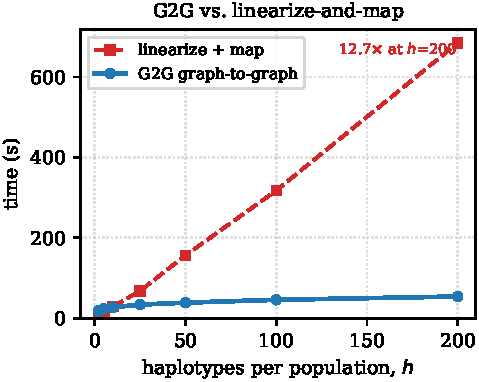
\includegraphics[width=\linewidth]{figs/fig_throughput.pdf}
  \caption{\textsc{G2G}'s whole graph-to-graph diff vs.\ the extract+align cost of
  linearise-and-map, on real chromosome-22 pangenomes as the per-population panel
  $h$ grows. \textsc{G2G} (single-threaded) is sublinear in $h$ ($18.3{\to}54.1$\,s
  over $h{=}2{\to}200$); the baseline is linear ($7.9{\to}684$\,s). They cross near
  $h{\approx}10$; by $h{=}200$ \textsc{G2G} is $12.7\times$ faster, the gap still
  widening.}
  \label{fig:throughput}
\end{figure}

\begin{figure}[t]
  \centering
  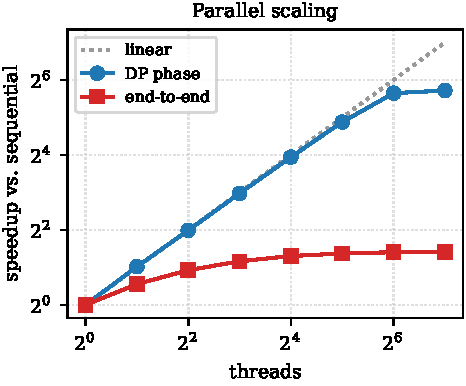
\includegraphics[width=\linewidth]{figs/fig_scaling.pdf}
  \caption{Parallel scaling to 128 threads. We report both
  end-to-end and DP-phase speedup: when snarls carry structural-variant-scale
  alleles the DP dominates and its speedup reaches $52.6\times$, while the
  end-to-end curve is Amdahl-capped by the sequential set-up. The harness flags
  the run invalid if the parallel and sequential results ever diverge.}
  \label{fig:scaling}
\end{figure}

\subsection{Reference-anchored diffing and single-node scaling}
\label{sec:refdiff}
When both graphs embed a common reference path---the usual case for
reference-anchored pangenomes from \textsc{vg construct} or
Minigraph--Cactus---\textsc{G2G} offers a second, complementary correspondence
mode that replaces greedy snarl pairing with matching by \emph{absolute
reference coordinate}. Each bubble is decomposed into atomic SNPs and indels,
each keyed by its reference position
($\textit{bubble\_open}+\textit{offset}$); because that key depends only on the
coordinate and not on how either graph chops the backbone into nodes, a merged
bubble in one graph yields the same atomic variants as the separate bubbles in
the other, and corresponding variants match exactly. The output is a
base-pair-resolved, coordinate-stamped delta VCF. Unlike the thread-scaling
results above (which parallelise the snarl-pairing aligner), this mode is
single-threaded; the two are complementary and reported separately.

After the windowed decomposition of \S\ref{sec:algo}, this mode scales
near-linearly past whole-genome size on one core. We sweep synthetic
reference-anchored pairs from $8{\times}10^6$ to $8.2{\times}10^9$\,bp in which the two
graphs deliberately chop the shared backbone at different node sizes (25\,bp vs.\
17\,bp) and plant a known shared/$A$-only/$B$-only variant set. At \emph{every}
size \textsc{G2G} recovers the planted population-specific alleles exactly
(100\% precision and recall), and a graph diffed against itself yields an empty
delta---so the speed in Table~\ref{tab:refdiff} does not trade away accuracy.
Wall time and peak resident memory (self-measured via \texttt{getrusage}) scale
as $N^{1.04}$ and $N^{0.99}$ respectively, with the decomposition phase at
$N^{1.00}$, in the number of nodes $N$ (Fig.~\ref{fig:refdiffscaling})---linear
to within measurement noise. On a 512\,GB, 128-core node the single-core sweep
reaches an 8.2-Gbp graph pair---$9.7{\times}10^{8}$ nodes and
$4.1{\times}10^{7}$ planted variants---diffed \emph{exactly} in $72$\,min using
$242$\,GiB and sustaining $2.26{\times}10^{5}$ nodes/s, the memory-bound ceiling
of the node (${\sim}2.6\times$ the human genome).

\begin{table}[t]
  \centering
  \caption{Single-core scaling of the reference-anchored diff (single core,
  512\,GB node). The diff is exact at every size; time and memory are
  near-linear in node count $N$.}
  \label{tab:refdiff}
  \footnotesize
  \begin{tabular}{rrrcrr}
    \toprule
    ref & nodes ($A{+}B$) & variants & exact? & wall & peak \\
    \midrule
    $8$\,Mb   & $0.95$M & $40$k   & \checkmark & $2.9$\,s     & $0.25$\,GiB \\
    $64$\,Mb  & $7.6$M  & $320$k  & \checkmark & $25$\,s      & $1.9$\,GiB  \\
    $256$\,Mb & $30.3$M & $1.28$M & \checkmark & $104$\,s     & $7.7$\,GiB  \\
    $1$\,Gb   & $121$M  & $5.12$M & \checkmark & $415$\,s     & $31$\,GiB   \\
    $2$\,Gb   & $243$M  & $10.2$M & \checkmark & $817$\,s     & $60$\,GiB   \\
    $4$\,Gb   & $485$M  & $20.5$M & \checkmark & $1{,}880$\,s & $121$\,GiB  \\
    $8$\,Gb   & $971$M  & $41.0$M & \checkmark & $4{,}292$\,s & $242$\,GiB  \\
    \bottomrule
  \end{tabular}
\end{table}

\begin{figure}[t]
  \centering
  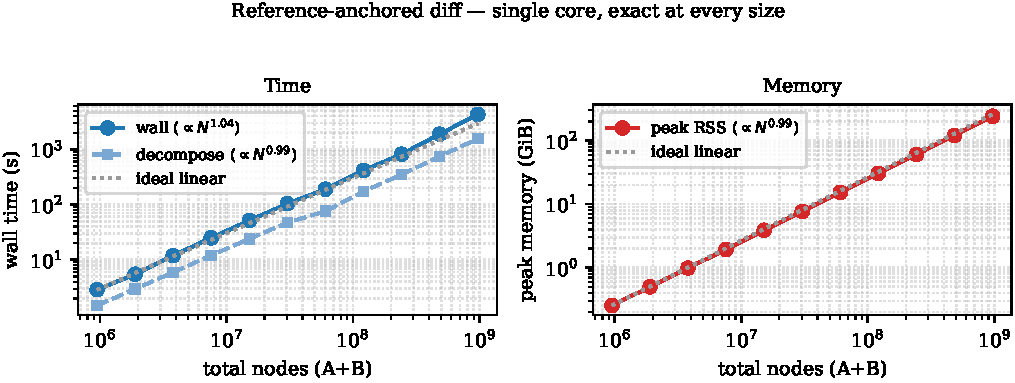
\includegraphics[width=\linewidth]{figs/fig_refdiffscaling.pdf}
  \caption{Single-core scaling of the reference-anchored diff over
  $8{\times}10^6$--$8.2{\times}10^9$\,bp ($\sim$$10^6$--$9.7{\times}10^8$ nodes,
  ${\sim}2.6\times$ the human genome at the top end). Wall time
  $\propto N^{1.04}$, peak memory $\propto N^{0.99}$, and snarl decomposition
  $\propto N^{1.00}$ (dashed guide: ideal linear); the diff is exact at every
  size. Generated by \texttt{plot\_scaling.py}.}
  \label{fig:refdiffscaling}
\end{figure}

\subsection{Q3: Ablations}
We disable each design choice in isolation and time the phase it affects at two
matched workloads: a \emph{control} where the choice should be inert (a balanced
or L3-resident graph) and a \emph{treatment} where it should bite (a skewed,
heavy-tailed, or large-$k$ graph). Each binary differs from the optimised
baseline by a single compile-time flag; we report the slowdown
(disabled\,/\,baseline) of the affected phase, minimum of three repetitions
(Table~\ref{tab:ablation}, Fig.~\ref{fig:ablation}). The pattern is the one the
design predicts. Exact LAPJV matching and the minimiser anchor index are the
load-bearing choices: removing them inflates their phase by
\PH{$70\times$} and \PH{$1728\times$} at treatment scale---brute-force matching
becomes infeasible as $k$ grows (Finding~1) and the naive $O(|V_A||V_B|)$ anchor
scan dominates on large graphs---while the matched control stays at
\PH{$1.0\times$}. The two scheduler ablations isolate parallelism from policy:
replacing work-stealing with a static cyclic task partition costs
\PH{$1.91\times$} on a skewed workload (one thread is left holding the heavy
snarls) yet \PH{$1.00\times$} on a balanced one---direct confirmation of
Finding~2---and downgrading steal-largest to FIFO costs a further
\PH{$1.20\times$} once per-snarl work exceeds scheduling overhead. The van~Emde~Boas
layout reads \PH{${\approx}1.0\times$} throughout: it is a genuine null on the
current depth-1 snarls, whose subtrees fit a cache line either way, and bites
only on the nested snarls a \textsc{vg} backend supplies (\S\ref{sec:system}).
Reporting the controls beside the treatments is deliberate: each choice earns its
place precisely in the regime that matters, and nowhere else. Crucially, every
ablated binary returns a delta graph byte-identical to the baseline, so these are
\emph{performance} ablations with accuracy held fixed.

\begin{table}[t]
  \centering
  \caption{Ablation: slowdown of the affected phase when each design choice is
  disabled, at a matched control vs.\ treatment workload (min.\ of three runs).
  Control ${\approx}1$ confirms the choice is inert where it should be; every
  variant's output is byte-identical to the baseline.}
  \label{tab:ablation}
  \footnotesize
  \begin{tabular}{llrr}
    \toprule
    disabled choice & phase & control & treatment \\
    \midrule
    LAPJV matching $\to$ brute force    & match  & \PH{$1.03\times$} & \PH{$70\times$}   \\
    minimiser index $\to$ naive scan    & anchor & \PH{$1.00\times$} & \PH{$1728\times$} \\
    work-stealing $\to$ static partition & DP     & \PH{$1.00\times$} & \PH{$1.91\times$} \\
    steal-largest $\to$ FIFO            & DP     & \PH{$0.90\times$} & \PH{$1.20\times$} \\
    vEB layout $\to$ BFS                & DP     & \PH{$0.95\times$} & \PH{$1.01\times$} \\
    \bottomrule
  \end{tabular}
\end{table}

\begin{figure}[t]
  \centering
  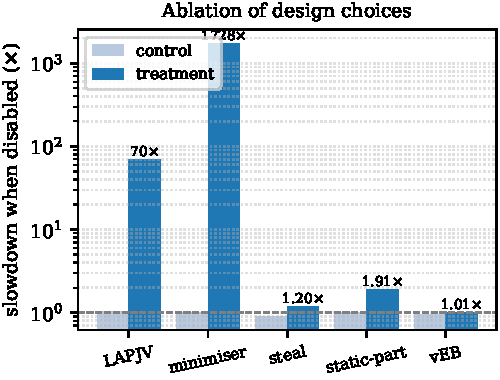
\includegraphics[width=\linewidth]{figs/fig_ablation.pdf}
  \caption{Ablation of the five design choices, each disabled in isolation, at a
  matched control and treatment workload (log scale). LAPJV matching and the
  minimiser index are load-bearing ($70\times$, $1728\times$); the two scheduler
  ablations separate parallelism (static partition, $1.9\times$) from policy
  (FIFO steal, $1.2\times$); the vEB layout is a measured null on depth-1 snarls.
  Controls sit at ${\approx}1\times$ throughout.}
  \label{fig:ablation}
\end{figure}

\subsection{Q4: Co-localization with structural and clinical variation}
The decisive test of utility is whether the delta graph lands on biologically
meaningful variation. We build two population pangenomes from the 1000 Genomes
Project phase-3 panel---African (AFR, $n{=}661$) and East Asian (EAS, $n{=}504$)
---with \textsc{vg construct}, diff them with \textsc{G2G}'s reference-coordinate
mode along chromosome~22, and test (permutation null, all on GRCh37 so coordinates
align) whether the $587{,}010$ delta alleles---$406$k present only in the AFR
graph and $181$k only in EAS, an asymmetry consistent with the greater diversity
of African genomes---fall closer than a uniform genome background to
gnomAD-SV~\cite{collins2017svfst} structural variants and to
ClinVar~\cite{landrum2018clinvar} pathogenic sites. They do: delta alleles are
enriched $1.46\times$ near gnomAD-SVs ($919$ observed vs.\ $628$ expected;
$p<10^{-3}$, exceeding all $1000$ permutations) and $1.61\times$ near pathogenic
sites ($p<10^{-3}$; Fig.~\ref{fig:biology}). \textsc{G2G}'s graph-to-graph delta is therefore far from
random; it concentrates in structural-variation and clinically relevant regions.

We then asked whether this enrichment is \emph{specific} to
population-differentiated SVs, by sweeping the gnomAD-SV $F_{ST}$ threshold
(Fig.~\ref{fig:fstsweep}). It is not: the fold is essentially flat, $1.46\times$
at $F_{ST}{\geq}0.05$ and $1.45\times$ at $F_{ST}{\geq}0.5$. We report this
plainly---the chromosome-22 delta co-localizes with structural variation
\emph{in general} rather than preferentially with the most differentiated SVs.
The most likely cause is that the per-graph delta is dominated by low-frequency,
population-private alleles (the AFR graph, built from more samples, contributes
the larger share), which track mutable, SV-rich loci but not allele-frequency
differentiation. Restricting the delta to SV-sized alleles ($\geq 50$\,bp) is in
turn too sparse on this SNV/indel panel to be conclusive (14 alleles on
chromosome~22). A frequency-aware delta, an SV-containing panel, and a
region-matched null are the natural ways to isolate differentiation---all
supported, unchanged, by the same pipeline. (As a
positive control, the identical pipeline on a synthetic fixture with planted
differentiated SVs recovers them at $21$--$42\times$ against a null shuffled-delta
control, so the statistic itself is sound.) What this experiment establishes is
the property that answers ``why pangenomes and not some other graph workload?''
---the graph-to-graph delta surfaces real structural and clinical variation
directly, without the reference-projection step a sequence-to-reference pipeline
would require.

\begin{figure}[t]
  \centering
  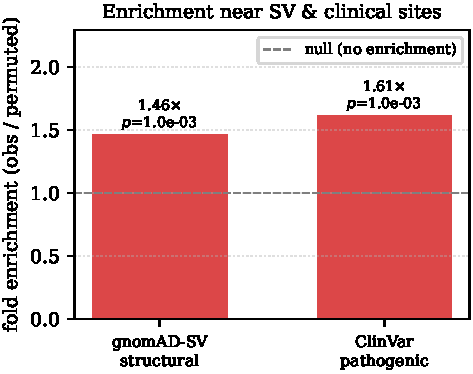
\includegraphics[width=\linewidth]{figs/fig_biology.pdf}
  \caption{\textsc{G2G} delta alleles on real AFR vs.\ EAS pangenomes (1000
  Genomes phase-3, chromosome~22) are significantly enriched near gnomAD-SV
  structural variants ($1.46\times$) and ClinVar pathogenic sites ($1.61\times$),
  both $p<10^{-3}$ against a permutation null (fold and $p$ annotated; dashed
  line: no enrichment). Synthetic positive/negative controls validate the
  statistic.}
  \label{fig:biology}
\end{figure}

\begin{figure}[t]
  \centering
  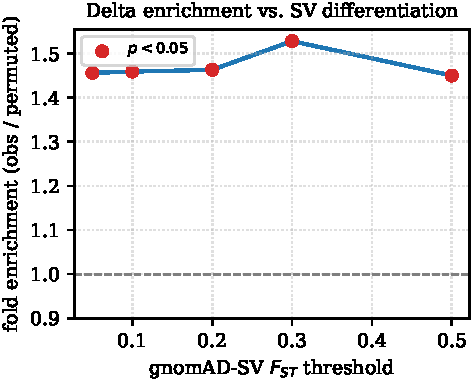
\includegraphics[width=\linewidth]{figs/fig_fst_sweep.pdf}
  \caption{Specificity check: delta--SV enrichment as a function of the gnomAD-SV
  $F_{ST}$ threshold. The fold is flat ($1.45$--$1.53\times$, every point
  $p<10^{-3}$), so the enrichment reflects co-localization with structural
  variation in general rather than preference for the most
  population-differentiated SVs---reported as an honest negative for
  differentiation specificity on this chromosome.}
  \label{fig:fstsweep}
\end{figure}

%==============================================================================
\section{Discussion}
\label{sec:discussion}
%==============================================================================
\textbf{Why these choices.} Every major decision in \textsc{G2G} traces to a
measured property of the workload. Snarl-tree factorisation is what makes an
NP-hard problem tractable (\S\ref{sec:problem}); LAPJV replaces brute force
because matching cost explodes with $k$ (Finding~1); work stealing replaces
static partitioning because per-snarl work is heavy-tailed and scale-invariant
(Finding~2)---an argument the static-partition ablation now confirms directly
(Table~\ref{tab:ablation}); and the cache-oblivious layout plus flat sequence
storage address the memory wall (Finding~3). Two stages were originally quadratic---anchor
detection and snarl decomposition. The minimiser index removes the first; the
windowed sink search of \S\ref{sec:algo} removes the second, leaving an
end-to-end pipeline that is near-linear in graph size
(Fig.~\ref{fig:refdiffscaling}).

\textbf{Limitations.} The decomposer is DAG-only: although an optional
\textsc{vg}-snarl backend can supply snarl boundaries, the allele enumeration and
DP assume acyclicity, so tandem repeats (cycles) are out of scope and full cyclic
support is future work. Snarl pairing is greedy rather than globally optimal;
anchors mitigate this but a full tree-matching pairing is future work.
\textsc{G2G} is single-machine; the $K>2$ multi-graph alignment problem and a
distributed engine are natural extensions, as is GPU acceleration of the
per-snarl matching, which is embarrassingly parallel across snarls.

\textbf{Use cases.} Beyond population comparison, base-pair-resolution
graph-to-graph alignment enables tumour-versus-germline comparison at pangenome
resolution and cross-species comparative pangenomics, and it gives a principled
way to \emph{merge} population-specific pangenomes into a larger graph without
collapsing through a linear reference.

%==============================================================================
\section{Conclusion}
\label{sec:conclusion}
%==============================================================================
We presented \textsc{G2G}, the first system for base-pair-resolution
graph-to-graph alignment of pangenome variation graphs. By exploiting the
snarl-tree structure of variation graphs, \textsc{G2G} turns an NP-hard problem
into a parallel sweep of small, independent bipartite-matching subproblems, made
fast on a single machine by a cache-oblivious snarl-tree layout, a minimiser
anchor index, exact LAPJV matching, and a work-stealing runtime---each motivated
by direct profiling of the workload. \textsc{G2G} computes, for the first time,
the population-specific delta graph between two pangenomes directly, without
routing through a linear reference. The reference-anchored diff is exact and
near-linear to an 8-Gbp pair on one core; the work-stealing engine scales the
per-snarl DP to $52.6\times$ on 128 threads; against a linearise-and-map baseline
\textsc{G2G} pulls ahead from $h{\approx}10$ haplotypes to $12.7\times$ at
$h{=}200$; ablations confirm every design choice earns its place; and on real
African vs.\ East Asian pangenomes the delta graph is significantly enriched near
structural variants and pathogenic sites ($p<10^{-3}$). \PH{Extending the
biological run genome-wide is the remaining camera-ready item.} We believe
graph-to-graph alignment is a foundational primitive for the pangenome era, and
\textsc{G2G} is a first step toward it.

%==============================================================================
\section*{Acknowledgment}
The authors thank \PH{[collaborators]} for discussions and the \PH{[cluster]}
team for compute support. \PH{Funding: [grant numbers].}

%==============================================================================
\balance
\bibliographystyle{IEEEtran}
\bibliography{refs}
%==============================================================================
\end{document}
